%%%%%%%%%%%%%%%%%%%%%%%%%%%%%%%%%%%%%%%%%%%%%%%%%%%%%%%%%%%%
%%% ELIFE ARTICLE TEMPLATE
%%%%%%%%%%%%%%%%%%%%%%%%%%%%%%%%%%%%%%%%%%%%%%%%%%%%%%%%%%%%
%%% PREAMBLE 
\documentclass[9pt,lineno]{elife}
% Use the onehalfspacing option for 1.5 line spacing
% Use the doublespacing option for 2.0 line spacing
% Please note that these options may affect formatting.
% Additionally, the use of the \newcommand function should be limited.


\usepackage{lipsum} % Required to insert dummy text
\usepackage[version=4]{mhchem}
\usepackage{siunitx}
\usepackage[export]{adjustbox}
\DeclareSIUnit\Molar{M}

\newcommand{\jdbcomment}[1]{\emph{\color{red} [#1]}}

%%%%%%%%%%%%%%%%%%%%%%%%%%%%%%%%%%%%%%%%%%%%%%%%%%%%%%%%%%%%
%%% ARTICLE SETUP
%%%%%%%%%%%%%%%%%%%%%%%%%%%%%%%%%%%%%%%%%%%%%%%%%%%%%%%%%%%%
\title{Single-cell virus sequencing of influenza variants that trigger innate immunity}

\author[1]{Alistair B. Russell}
\author[1,2,3*]{Jesse D. Bloom}
\affil[1]{Basic Sciences Division and Computational Biology Program, Fred Hutchinson Cancer Research Center, Seattle, United States}
\affil[2]{Department of Genome Sciences, University of Washington, Seattle, United States}
\affil[3]{Howard Hughes Medical Institute, Fred Hutchinson Cancer Research Center, Seattle, United States}

\corr{jbloom@fredhutch.org}{JDB}

%%%%%%%%%%%%%%%%%%%%%%%%%%%%%%%%%%%%%%%%%%%%%%%%%%%%%%%%%%%%
%%% ARTICLE START
%%%%%%%%%%%%%%%%%%%%%%%%%%%%%%%%%%%%%%%%%%%%%%%%%%%%%%%%%%%%

\begin{document}

\maketitle

\begin{abstract}
The outcome of viral infection is extremely heterogeneous at the cellular level, and many viruses trigger innate immunity in only a fraction of infected cells. 
Here we develop an approach to determine how the genetic variation inherent in viral populations contributes to this heterogeneity.
We simultaneously determine the cellular transcriptome and full sequences of all viral genes in hundreds of influenza-infected cells.
Infections that trigger immunity are associated with several features: absence of the gene encoding the virus's primary immune antagonist, internal deletions in viral polymerase genes, and point mutations in viral proteins involved in replication and nuclear export. 
However, immune activation remains stochastic in cells infected by viruses with these genetic lesions, and sometimes occurs even in cells infected with fully wildtype virions.
Overall, our work shows that viral genetic variation substantially contributes to but does not fully explain heterogeneity in infection outcome and immune activation.
\end{abstract}


\section{Introduction}

\citep{russell2018extreme} and \citep{steuerman2018dissection}.

\clearpage
\section{Results}

\subsection{A method to obtain the complete genotypes of the virions infecting single cells that do and do not express IFN}

Two challenges:

IFN expression is rare in infected cells (\FIG{IFNrare}).
Apparent in single-cell \textit{in vitro}~\citep{russell2018extreme}, single-cell \textit{in vivo}~\citep{steuerman2018dissection}, and reporter assays by others~\citep{killip2017single} and ourselves (\FIG{IFNrare}).

%%% start IFNrare figure %%%
\begin{figure}
\centerline{
{\bf \Large A}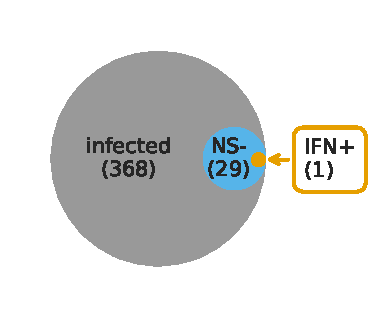
\includegraphics[width=0.25\textwidth,valign=t]{figures/IFN_stochastic/RussellVenn/venn_diagram.pdf}
{\bf \Large B}
}
\caption{
Triggering of IFN production is rare in influenza-infected cells.
{\bf (A)} Number of influenza-infected and IFN+ cells in our prior single-cell study of influenza infection of A549 cells.
The Venn diagram shows data aggregated over all samples from \citet{russell2018extreme}.
{\bf (B)} An A549 fluorescent-reporter cell-line confirms that IFN expression is rare in cells infected with our viral stock.
\jdbcomment{This should be a simple figure, such as a plot that just shows the fraction IFN+ among flu infected cells for a few replicates.
If you have suitable data, you could show for low, medium, and high-inducing stock and indicate which we use.
Then put detailed flow data similar to what is in your writeup in \FIGSUPP[IFNrare]{flow}. For that flow data, I think contour plots are better than overplotting. Also, don't subsample but show all points, as that will give better statistics.
We could possibly add a \emph{small simple} schematic of reporter line here as panel {\bf (B)} and move the current {\bf (B)} to {\bf (C)}, and then have more details in \FIGSUPP[IFNrare]{reporter_cells}.
Alternatively, we could just show everything in \FIGSUPP[IFNrare]{reporter_cells}.}
}
\label{fig:IFNrare}

\figsupp[Creation and validation of A549 fluorescent-reporter cell lines for type I and type III IFN expression.]
{CAPTION}
{\jdbcomment{ADD FIGURE}}
\label{figsupp:reporter_cells}

\figsupp[Expression of type I and type III IFN are highly correlated in influenza-infected A549 cells. \jdbcomment{Alternatively, we could leave this out if you don't have clean data for this point and just refer to \FIGSUPP[experiment]{type_I_III_correlation}}]
{CAPTION}
{\jdbcomment{ADD FIGURE}}
\label{figsupp:type_I_vs_III}

\figsupp[Full flow cytometry data for \FIG{IFNrare}B.]
{CAPTION}
{\jdbcomment{ADD FIGURE}}
\label{figsupp:flow}

\figsupp[Few cells express detectable IFN in the single-cell analysis influenza-infected mice by \citet{steuerman2018dissection}.]
{A re-analysis of the data from \citet{steuerman2018dissection}'s single-cell mRNA-sequencing of cells from influenza-infected mice shows that only 5 of 1220 virus-infected cells express \emph{detectable} type I or type III IFN transcripts \textit{in vivo}.
Specifically, we downloaded the data from \citet{steuerman2018dissection} and identified influenza-infected cells using calling criteria similar to those described in \citet{steuerman2018dissection}.
Here we show statistics for the cells from the influenza-infected wildtype C57BL/6J mice, which were collected at 48 hours (two replicates) or 72 hours (one replicate)---we do not show cells from the control mice.
As shown in the left-most panel, the sequencing depth of \citet{steuerman2018dissection} was quite low, with only $\sim$1,500 mRNA counts per cell on average (this is 10 to 15-fold lower than the sequencing depth in \citet{russell2018extreme} and the current study, respectively).
An important caveat is that this low sequencing depth could lead to a simple failure to detect IFN transcripts in some cells.
Nonetheless, there is detectable expression of key interferon-stimulated gene (ISG) mRNAs in the majority of infected cells (the middle panel shows the total counts of IFIT1, ISG15, CCL5, and Mx1).
However, only 5 of 1220 cells express any detectable type I (IFN-$\alpha$ and IFN-$\beta$) or type III (IFN-$\lambda$) mRNAs, and only at low levels.
The full code that performs the re-analysis shown in this figure is at \url{https://github.com/jbloomlab/IFNsorted_flu_single_cell/tree/master/paper/figures/IFN_stochastic/SteuermanReanalysis/}.
}
{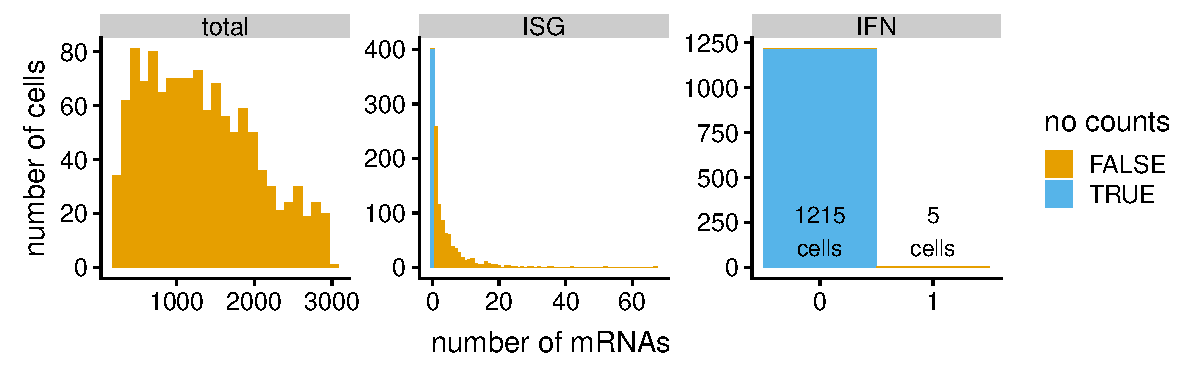
\includegraphics[width=\textwidth]{figures/IFN_stochastic/SteuermanReanalysis/plots/p_mRNA_counts.pdf}}
\label{figsupp:mice}

\end{figure}
%%% end IFNrare figure %%%

All past single-cell transcriptomics of viral infected cells~\citep{russell2018extreme,zanini2018single,steuerman2018dissection,zanini2018virus} have focused on counting the number of viral transcripts rather than determining their full sequences.
We came up with a scheme to determine full genotypes of infecting viruses in IFN+ cells (\FIG{experiment}).

%%% start approach figure
\begin{figure}
\begin{fullwidth}

{\centering
{\bf A} \jdbcomment{PANEL WITH EXPERIMENTAL OUTLINE SCHEMATIC} \vspace{0.2in}\\

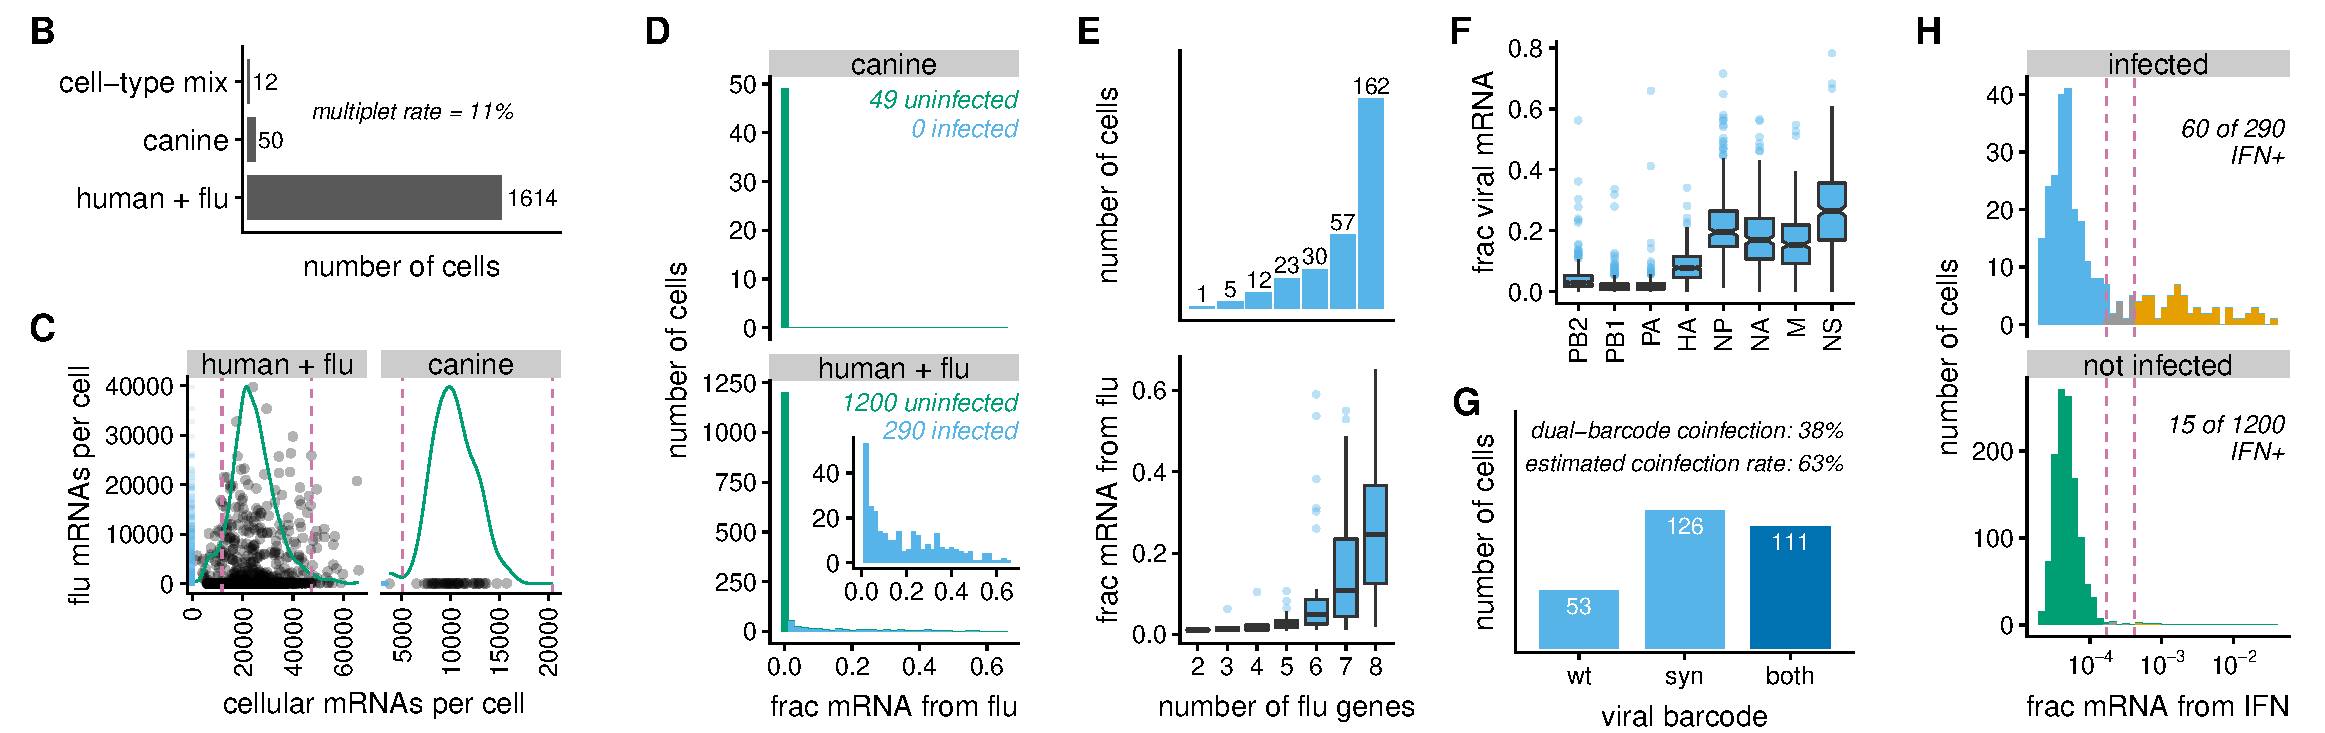
\includegraphics[width=\linewidth, clip=false]{figures/single_cell_figures/p_cell_summary.pdf}
}

\caption{
Experimental overview.
{\bf (A)} Schematic of approach.
{\bf (B)} Number of cells for which transcriptomes were obtained.
Most transcriptomes are from human cells, but a few are from the uninfected canine cells spiked into the experiment as a control.
From the transcriptomes with both human and canine transcripts, we estimate~\citep{bloom2018estimating} that $\approx$11\% of the captured cells are actually multiplets in which more than one cell was captured in an emulsion. 
These cross-celltype multiplets are excluded from subsequent analyses.
{\bf (C)} The number of cellular and viral mRNAs detected for each cell is plotted as a point.
Green lines show the distribution of cellular mRNAs per cell, and the blue rug plot at the left of each panel shows the distribution of viral mRNAs per cell.
Cells outside the dashed magenta lines have unusually low or high amounts of cellular mRNA (possibly low-quality emulsions or multiplets), and are excluded from subsequent analyses.
{\bf (D)} Distribution across cells of the fraction of all mRNA derived from influenza.
Cells called as infected are in blue, while other cells are in green.
The inset shows the amount of viral mRNA among the human cells called as infected.
{\bf (E)} The number of influenza genes detected per infected cell, and the amount of viral mRNA in cells expressing each number of viral genes.
The majority of cells express all eight gene segments, but a substantial minority fail to express at least one gene.
\FIGSUPP[experiment]{frac_has_gene} shows the frequency that each viral gene is detected in infected cells.
{\bf (F)} Relative expression of viral genes among infected cells.
{\bf (G)} The number of cells infected with wildtype virus, synonymously barcoded virus, or both.
From the cells infected with both viral barcodes, we estimate~\citep{bloom2018estimating} that 63\% of infected cells are co-infected.
{\bf (H)} Fraction of cellular mRNA derived from type I or type III IFN across all cells, faceted by whether the cells are infected.
Cells to the left of the first dashed magenta line are classified as IFN-, and cells to the right of the second line are classified as IFN+.
We grouped type I and type III IFN together because their expression is highly correlated (\FIGSUPP[experiment]{type_I_III_correlation}).
Many cells that do not express IFN itself still express interferon-stimulated genes (\FIGSUPP[experiment]{ISG}).
}
\label{fig:experiment}

\figsupp[Fraction of infected cells that detectably express each influenza gene.]
{Bars show the fraction of infected cells that are called as expressing each viral gene.
The gray dashed line is at one (the fraction that would be observed if all viral genes are expressed in all infected cells).
Each viral gene is detected in $\approx$80-90\% of the infected cells, roughly in line with prior estimates~\citep{brooke2013most, heldt2015single, dou2017analysis, russell2018extreme}.
The exception is NP, which is detected in virtually all infected cells.
The much higher frequency of detecting NP could reflect a biological phenomenon, or it could be because cells lacking NP tend to have much lower viral gene expression overall and so are not reliably called as being infected in our experiments and analysis.}
{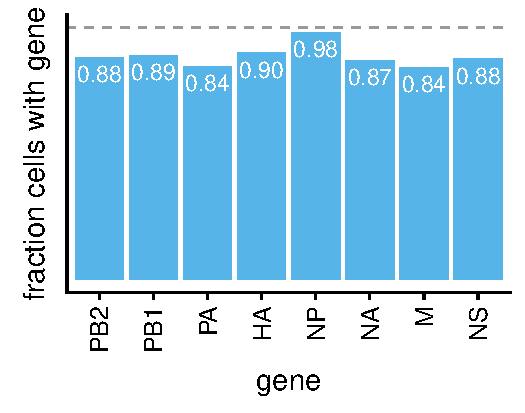
\includegraphics[width=0.5\textwidth]{figures/single_cell_figures/p_frac_has_gene.pdf}}
\label{figsupp:frac_has_gene}

\figsupp[Expression of type I and type III IFN genes is highly correlated in single cells in our experiments.]
{The correlation between the fraction of cellular mRNA derived from type I (IFN-$\alpha$ and IFN-$\beta$) and type III (IFN-$\lambda$) IFN in the A549 cells in our experiments.
Each point represents a single cell.
The plots are faceted by whether the cells are called as infected, and the Pearson correlation coefficient is shown.
Because type I and type III IFN expression are highly correlated, for the remainder of the paper we group them together and refer to their combined expression as the level of IFN.
}
{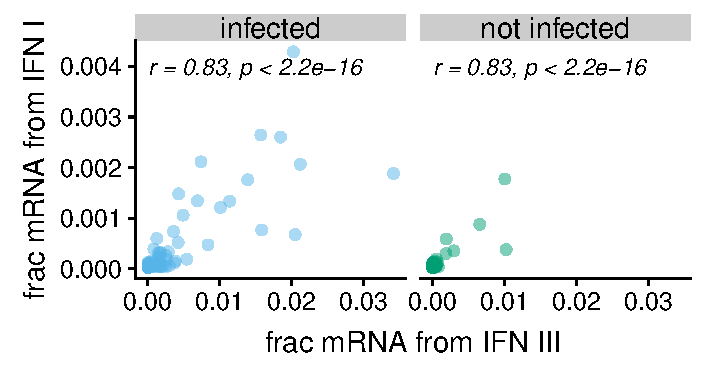
\includegraphics[width=0.7\textwidth]{figures/single_cell_figures/p_ifn_genes_corr.pdf}}
\label{figsupp:type_I_III_correlation}

\figsupp[Expression of interferon-stimulated genes (ISGs).]
{
For each cell, we quantified ISG expression as the total fraction of cellular mRNAs derived from four prototypical ISGs that are highly expressed A549 cells (IFIT1, ISG15, CCL5, and Mx1). 
{\bf (A)} The histograms show the distribution of ISG expression taken across infected (top) and uninfected (bottom) cells.
We heuristically classify as ISG+ cells with $>10^{-3}$ of their cellular mRNA from ISGs, and color these cells red.
Comparison to \FIG{experiment}H shows that substantially more cells are ISG+ than IFN+, both among infected and uninfected cells.
This is probably because paracrine signaling leads to ISG expression in some cells that are not themselves expressing IFN.
{\bf (B)} The correlation between the fraction of cellular mRNA derived from IFN and from ISGs.
Each point represents a single cell, and the Pearson correlation coefficient is shown.
IFN and ISG expression is more correlated for infected than uninfected cells, probably because in the latter the ISG expression is often due to paracrine signaling that does not induce expression of IFN itself.
But among both the infected and uninfected populations, there are many cells with high expression of ISGs and little expression of IFN, but very few cells that express high levels of IFN without also substantially expressing ISGs.
}
{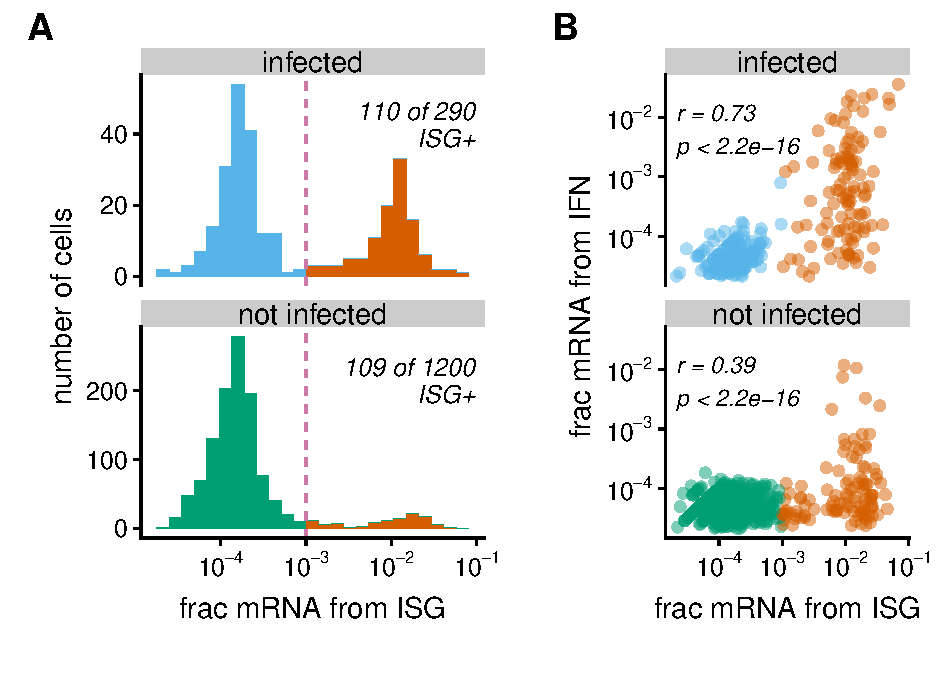
\includegraphics[width=0.8\textwidth]{figures/single_cell_figures/p_isg.pdf}}
\label{figsupp:ISG}

\figsupp[Unsupervised t-SNE clustering shows that cell-to-cell variation in influenza genes, IFN genes, and ISGs explains a substantial part of the structure of the data.]
{To generate an unbiased representation of the factors that distinguished the transcriptomes of the cells in our experiments, we used unsupervised t-SNE~\citep{maaten2008visualizing} as implemented in \texttt{Monocle}~\citep{qiu2017reversed, trapnell2014dynamics} to generate a two-dimensional representation of the data.
In the t-SNE plot, each point is a different cell and cells with similar transcriptomes are closer together.
Each panel shows the same t-SNE plot, but the cells are colored differently in each panel based on the amount of viral, IFN, or ISG mRNA shown on a log (top) or linear (bottom) scale.
As is clear from this plot, expression of influenza genes, IFN, and ISGs help explain the structure of the data, since cells with high expression of these genes clearly group together.
}
{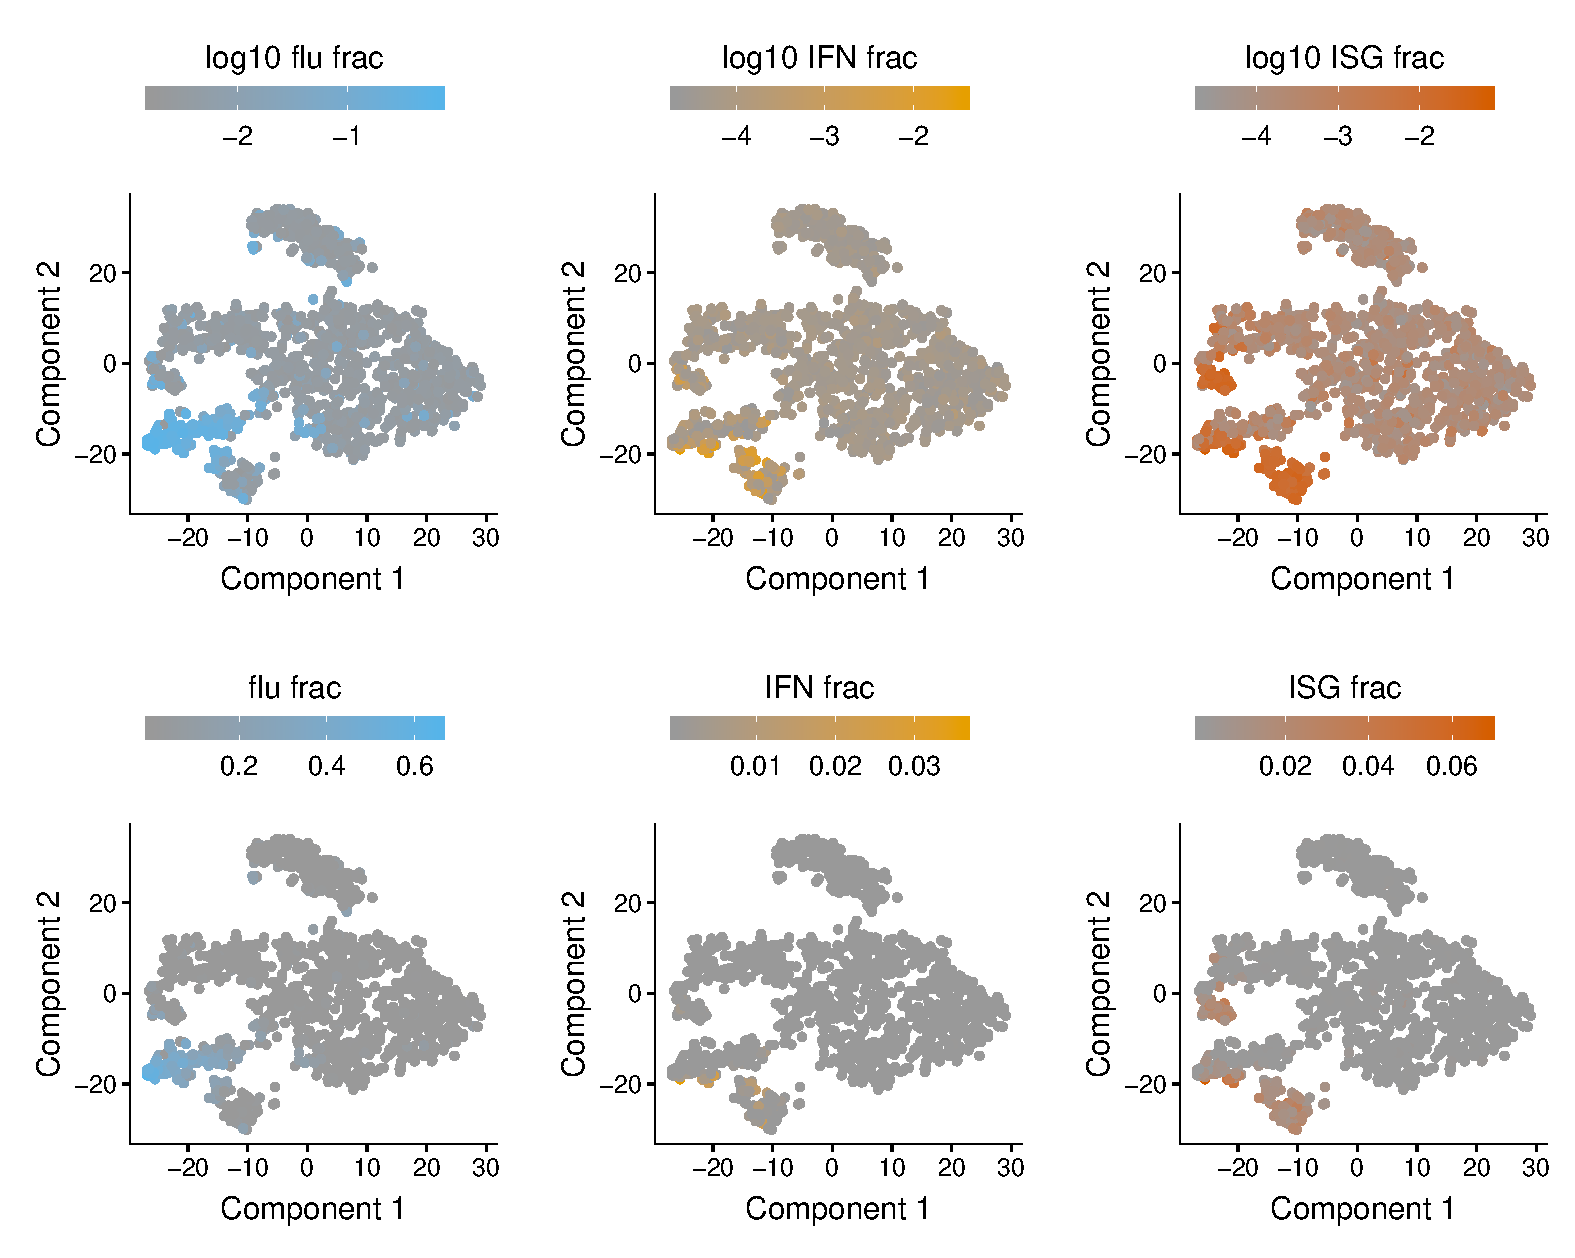
\includegraphics[width=\textwidth]{figures/single_cell_figures/p_tsne.pdf}}
\label{figsupp:tSNE}

\end{fullwidth}
\end{figure}
%%% end approach figure


\subsection{Viral genotypes in IFN+ and IFN- influenza-infected cells}
\FIG{genotypes} and \FIGSUPP[genotypes]{genotypes_by_ifn} and \FIGDATA[genotypes]{genotypes}


%%% start genotypes figure %%%
\begin{figure}
\begin{fullwidth}
{\centering
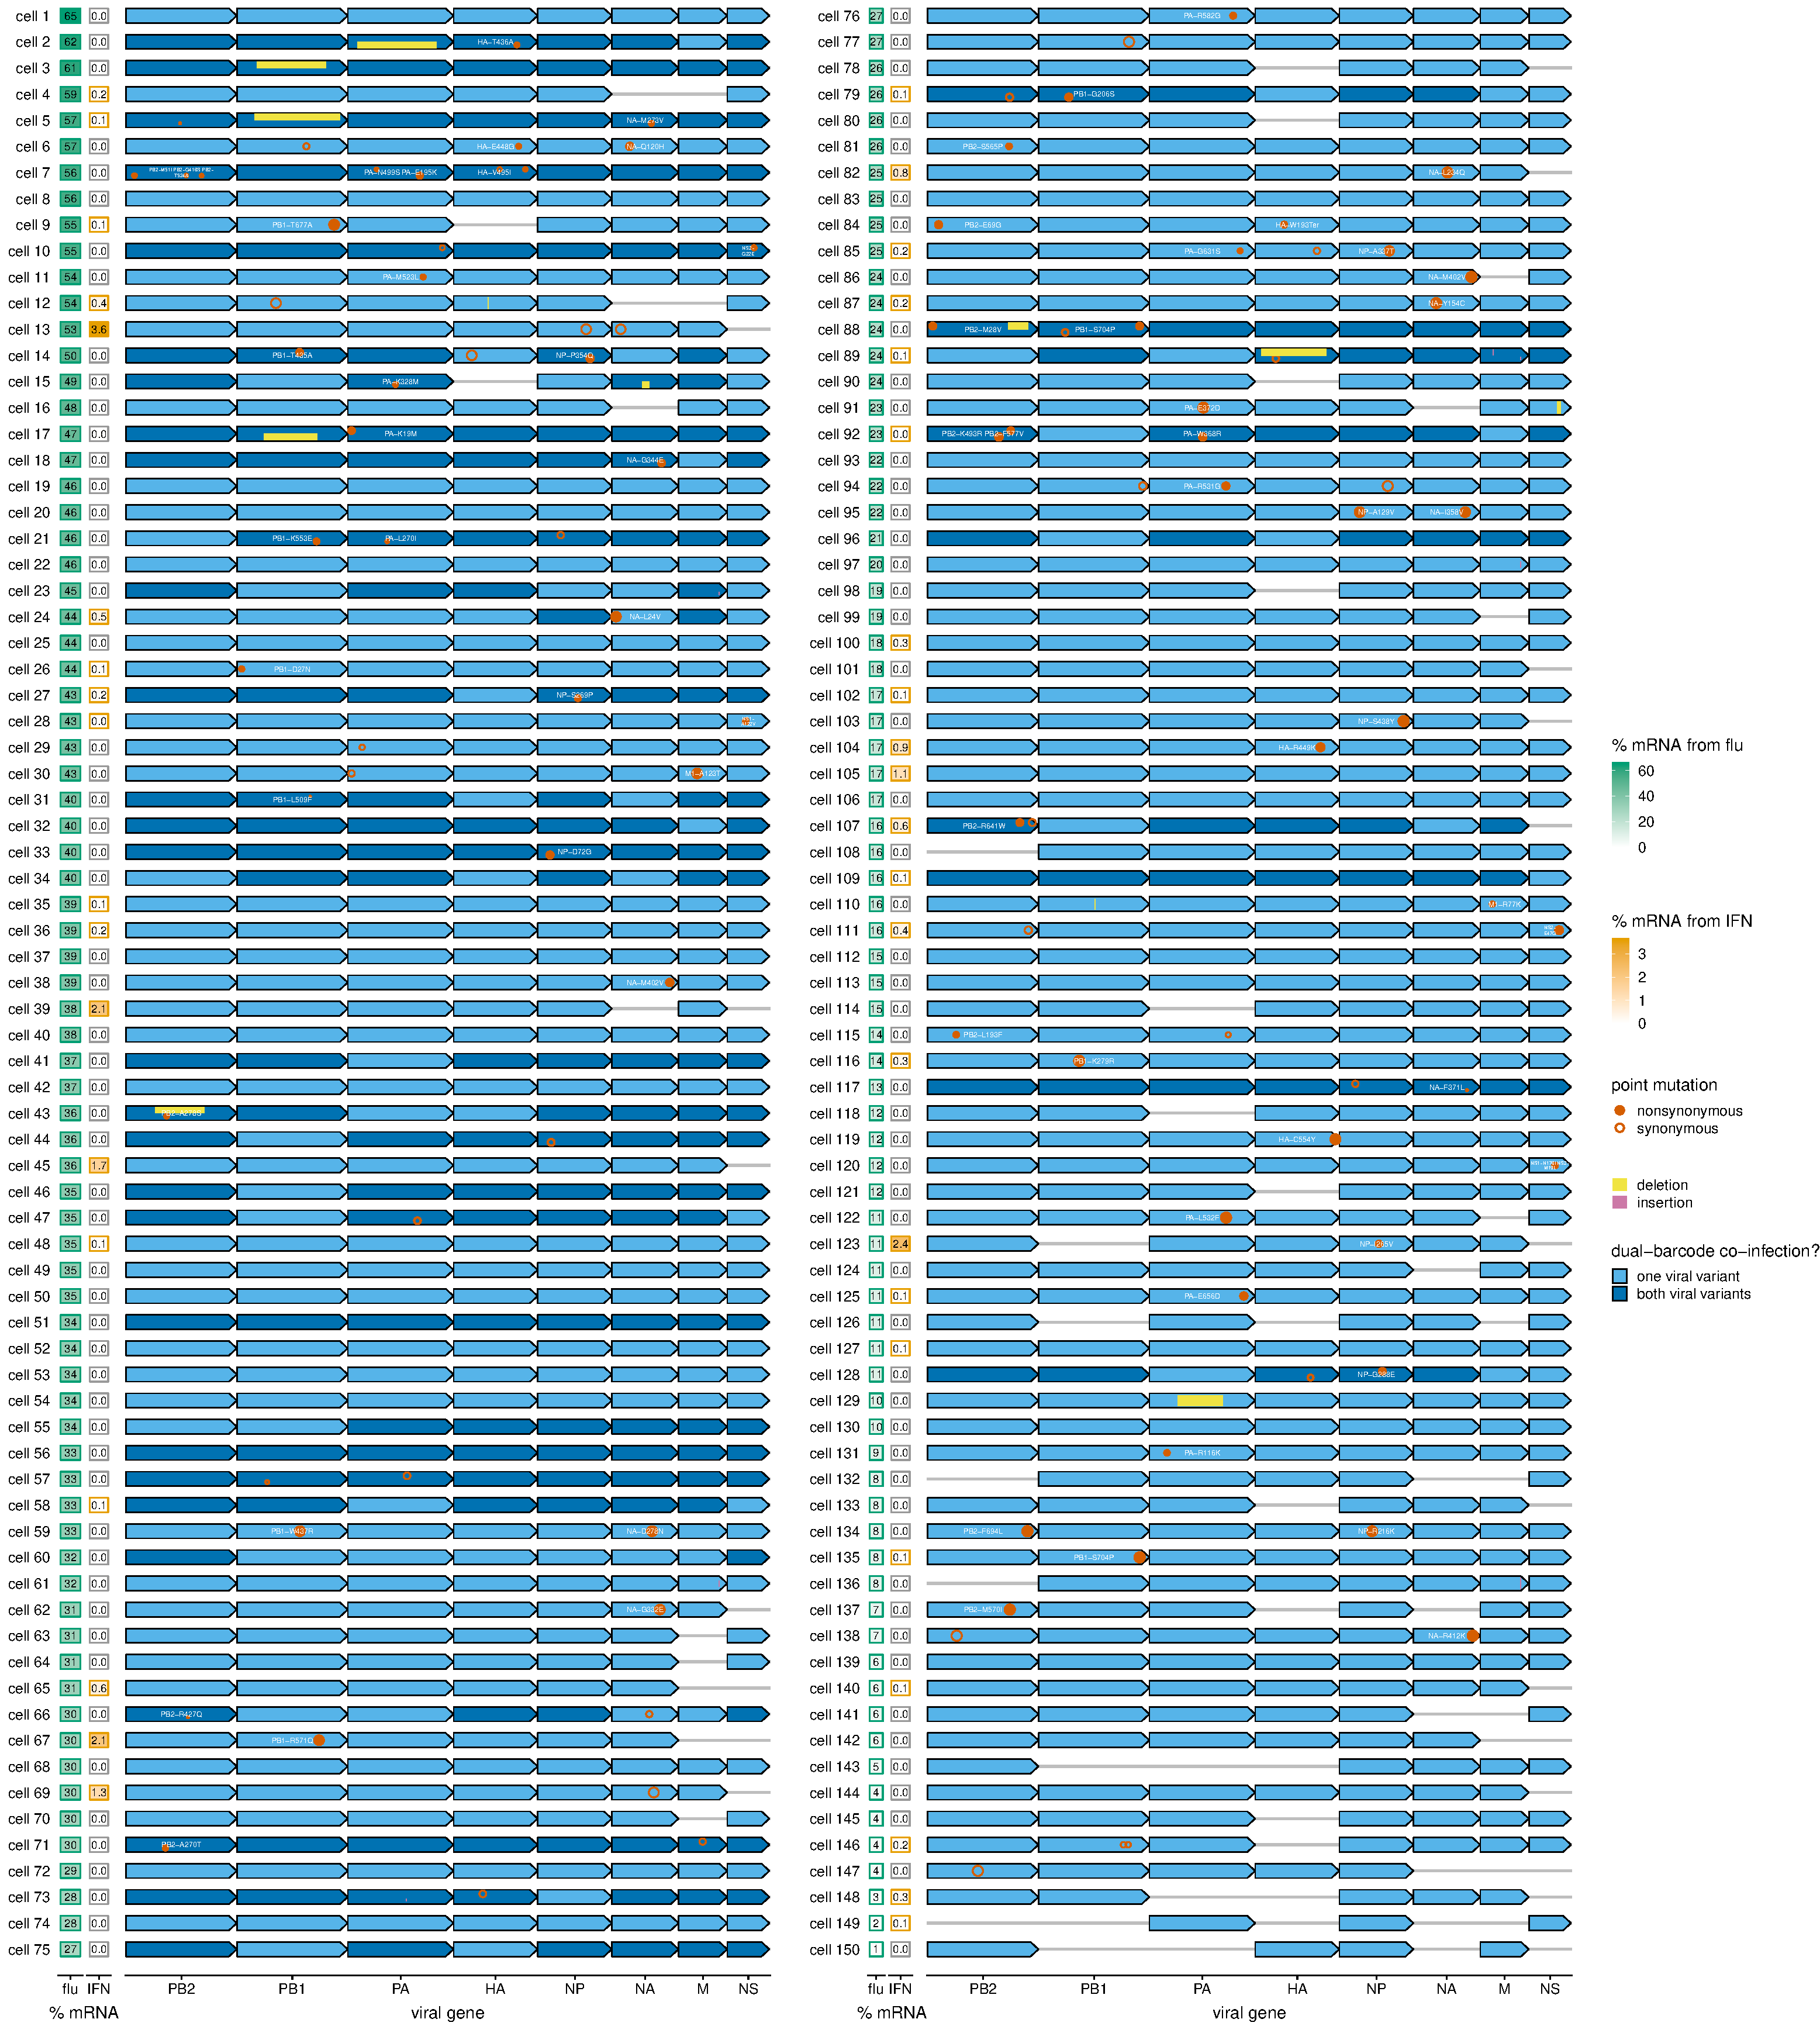
\includegraphics[width=0.9\linewidth]{figures/single_cell_figures/p_genotypes.pdf}
}
\caption{
Viral genotypes and infection outcomes in single cells.
}
\label{fig:genotypes}

\figsupp[Genotypes and infection outcomes plotted separately for IFN+ and IFN- cells.]
{This plot shows the same data as \FIG{genotypes}, but with cells separated into columns based on whether they are IFN- (left column) or IFN+ (right column).}
{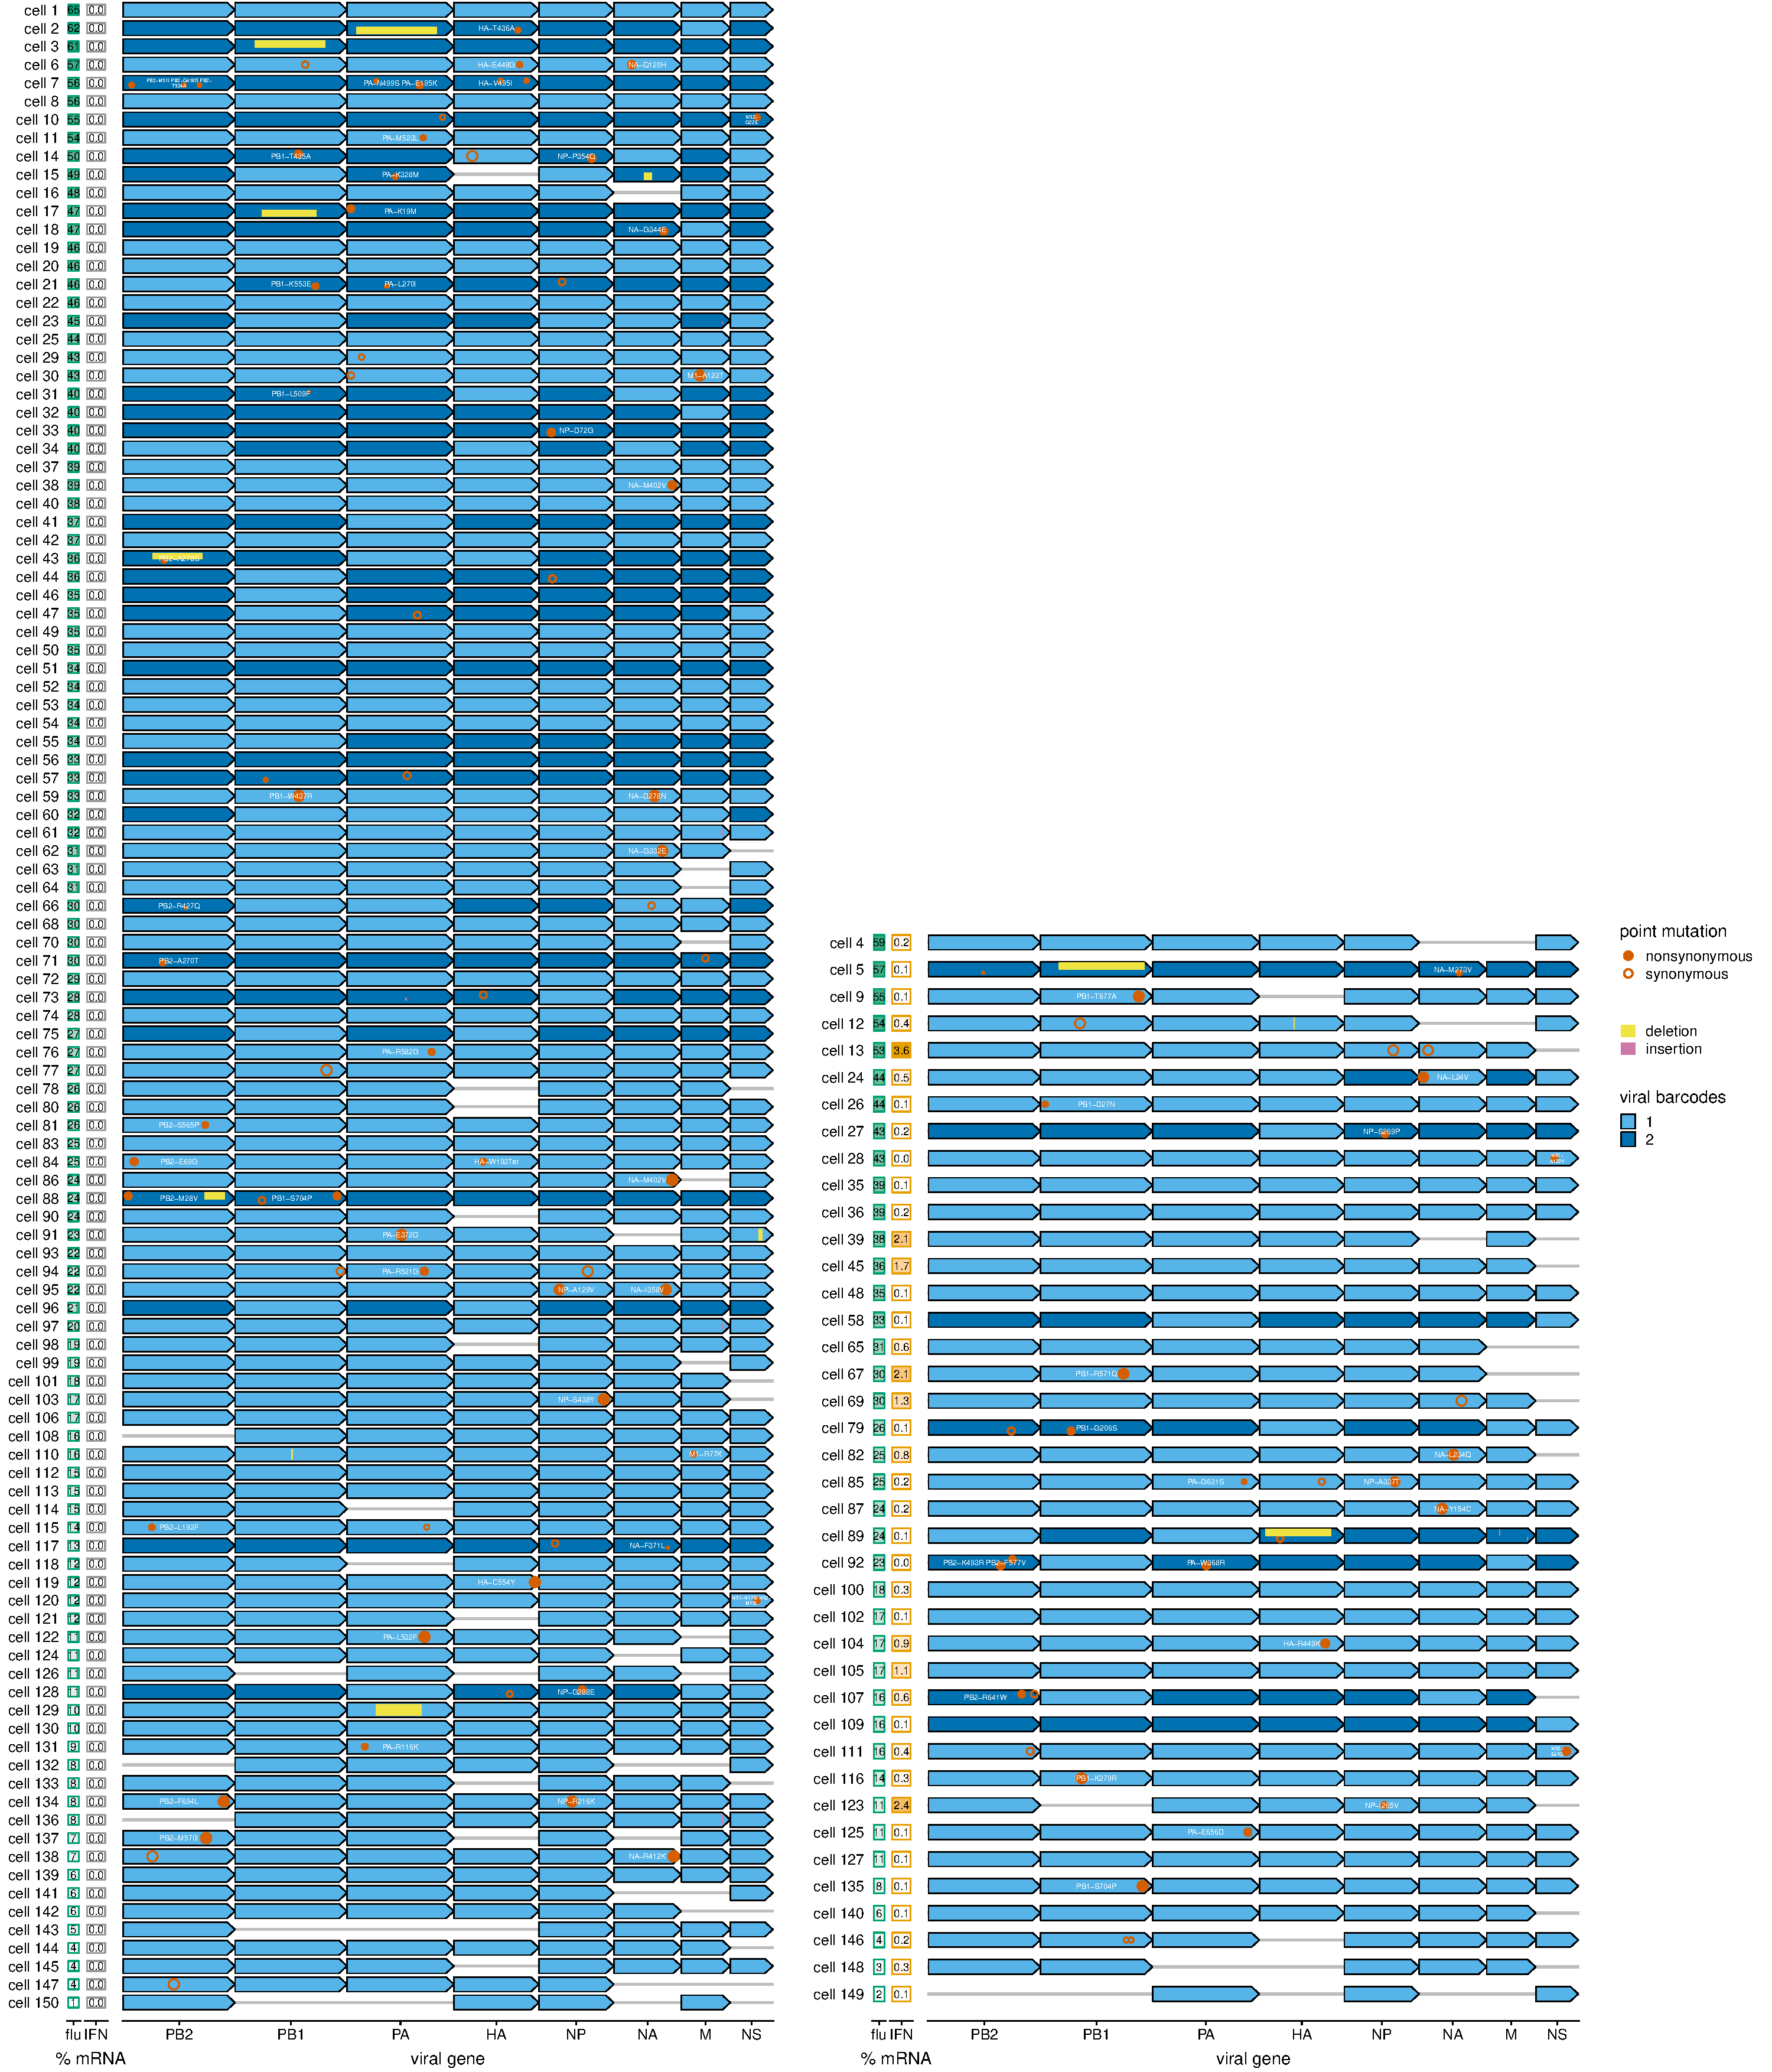
\includegraphics[width=\textwidth]{figures/single_cell_figures/p_genotypes_by_ifn.pdf}}
\label{figsupp:genotypes_by_ifn}

\figdata{A CSV file giving the genotypes is in \texttt{figures/single\_cell\_figures/genotypes.csv}.}
\label{figdata:genotypes}

\end{fullwidth}
\end{figure}
%%% end genotypes figure %%%

\section{Discussion}

Add text

\section{Methods and Materials}

Add text




\section{Acknowledgments}

Add this

\nolinenumbers

\bibliography{references}

\end{document}
